\section{Introduction}
\label{sec:intro}

%\begin{figure}[t]
%  \begin{center}
%    
\includegraphics[width=0.95\columnwidth]{figs/workflow.eps}
%    \caption{Workflow}
%    \label{fig:Normal workflow for most multi-tier service oriented systems}
%  \end{center}
%\end{figure}

\begin{figure*}[ht]
  \begin{center}
    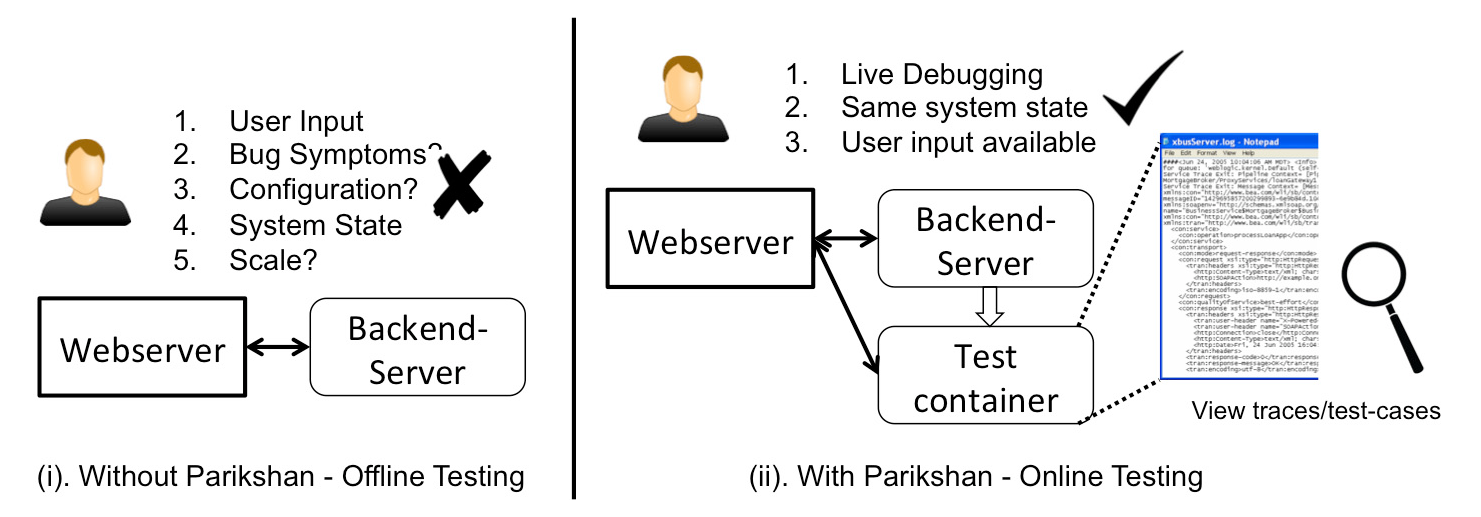
\includegraphics[width=0.7\textwidth]{figs/motivation.eps}
    \caption{Here (i). shows a workflow of a simple 2 tier system without \parikshan where the user has to do offline debugging, and will have to figure out someway to capture the user input/bug symptoms/system state, (ii) is the same system running with \parikshan, which allows the user to do online debugging in a parallel test-container cloned from the back-end server, which receives the same input}
    \label{fig:motivation}
  \end{center}
\end{figure*}


As application software grows and gets more complicated, testing large scale applications has become increasingly important. 
%This problem is compounded by the recent trend in software engineering industry by large companies towards DevOps\cite{devops}. 
The recent trend towards DevOps\cite{devops} by the software engineering industry further compounds this problem by requiring a fast and rapid resolution towards any software bug.
DevOps stresses on close coupling between software developers and operators, and to merge the operations of both. 
Most of these companies have very frequent releases and hence require a very short time to a bug fix, test, patch and release in order to realize continuous delivery(Facebook mobile has 2 releases a day, and Flickr has 10 deployment cycles per day).

However, it is extremely difficult to meet the quick debugging demands of a devops environment, as it is not feasible to recreate realistic workloads in an offline development environment for large scale multi-tier or cloud based applications.
In general, debugging in the development environment can be (1). Unrealistic because it may not be possible to faithfully reconstruct the production environment, (2). Incomplete, as it may be impossible to generate all possible input cases (3). Costly, as it is unfeasible to test all possible configurations given time and cost constraints of releasing the software to the field. 
Hence debugging is not only difficult because of difficulty to recreate production scenarios, it is also increasingly important to localize and fix bugs in a very short period of time.

One of the proposed mechanisms of addressing this problem is to ``perpetually test''\cite{perpetual} the application in the field after it has been deployed. 
This is important since testing in a production system enables us to capture previously ``unreachable'' system states, which can arise due to various factors such as unpredictable user environment, outdated software, an ever increasing list of hardware devices (e.g. mobile phones, embedded devices etc.), or simply because of imperfect network connectivity (wifi, cellular).
%which are possible only for a long running production environment. 
%Since we are testing in a real environment, we get real user-input for test-cases, and are able to test a real environment.
%However, perpetual testing has never gotten much traction because of an obvious flaw : executing such test-cases will adversely effect the user-experience, both in performance and potentially in application logic.
Some approaches such as Chaos Monkey\cite{chaosmonkey} from Netflix, and AB Testing\cite{abtesting} already use ``testing in the wild'' to check for errors and robustness of the software, or to check for new features that have been added.  
However, despite a clear need, testing in the wild has never gotten much traction in real-world applications as it consumes too much performance bandwidth and more importantly, it can affect the sanity\footnote{The state of the production server may change leading to a crash or wrong output} of real operational state of the software.
%Another trend embraced by mainstream companies such as Flickr, Twitter, Facebook and Google is DevOps\cite{devops}. 
%And wile testing, analyzing and monitoring are an important aspect of the devops cycle, usually only a very small performance bandwidth in the production server can be dedicated to QA operations as compared to real user activity(so as to not effect user-perceived delay). 

%Embedding test-case logic within the context of the application will result in state-change, or performance slow-down that would otherwise not be there in an optimized implmentation of the application.
%This is something which is usually unacceptable in user-facing applications.
%The authors have previously looked into amortizing the cost of running the test, by running it in parallel \cite{invite}.
%However such approaches cannot completely avoid the slowdown, and additonally do not completely sandbox the effects of the test case on the production server. 

%An alternate approach is to record live applications, and replay them offline.
%Over the years there have been several systems which have explored this direction with promising results.
%However most record and replay systems have high overheads, and require replication of the running configuration which may not be possible. 
%Additionally the administrator needs to wait for offline analysis, instead of doing real-time diagnosis.

%On the other hand, there has been an impressive increase in the scale of computing resources, and distributed scalability of infrastructure.
%Web based applications are often hosted in cloud environments, this allows for easily scaling up the hardware resources.
%This often allows for redundant computation, which can be used for testing purposes. 

The main reason that debugging in the development environment is easier, is because developers can trace the execution flow of the program using tools such as gdb\cite{gdb}, valgrind\cite{valgrind} etc. and look at variable values for the given input. 
This gives them an immediate insight as to whether the application is behaving correctly, and where the bug could be.
Unfortunately, such techniques are not possible in the production environment as they would lead to unacceptable slow-down, alter the application functionality, or worse crash the application.
The motivation behind our work is to provide \textbf{``bug diagnosis as a service''} for real-time debugging of production applications in order to significantly reduce the time towards bug resolution.
We observe that most modern day service oriented applications are hosted on IAAS cloud providers, and can hence be easily scaled  up. 
Leveraging this abundance of resources, and recent advances in user-space virtualization technology(OpenVZ/LXC\cite{openvz,lxc}) we present a debugging mechanism which allows the user to dynamically insert probes in a \emph{cloned} production environment without effecting the actual application: thereby, enabling real-time diagnosis.

 Our system called \parikshan\footnote{Parikshan is the Sanskrit word for testing} allows capturing the context of application, 
for tests to be run without effecting the sanctity and performance of the actual user-facing application. 
This is done by cloning a production server and creating two containers: a production container, and a testing container. 
We duplicate the incoming traffic to both the production container and the test container using a custom proxy, which ignores the responses from the test-container. 
The debugging on the test-container is done on the fly using dynamic instrumentation, hence any set of test-cases can be turned on whenever required. 
%This is achieved by using dynamic instrumentation mechanisms to clone a VM by forking off from a running executed state and encapsulating the forked execution in a VM.
%The user can pre-define probe points for dynamically inserting test-cases (by default the entry and exit of each function is considered a probe point).
Since the test is executed in a container it acts like a sandbox which restricts it from causing any perturbation to the state of the parent process, or effecting the sanity of the responses to the production client. 
We clone the production and test containers using a variant of live migration without suspending the services of the production server, and follow it up with frequent synchronization for long running tests.

%\textit{Parikshan}
%We provide a flexible framework which allows user access to a parallel test-container which behaves identically as the production container. 
While we discuss several case-studies to debug/ test production applications that show how our framework can be used, we wish to stress that \textbf{the main advantage of \parikshan is a harness/ framework for testing/ debugging in a live environment rather than a new testing methodology}. 
The key contributions of this paper are:

\begin{itemize}

\item A tool which provides a sandbox environment to debug the production environment. 
This allows for a safe and secure mechanism to perturb and diagnose the application, \textbf{without effecting the functionality} of the  production container.

\item A testing harness, and proxy which ensures non-blocking request duplication to the test-container, which ensures \textbf{no performance impact} on the production container. 

\item Our tool tracks the \textbf{fidelity of the test-container} ( if the test-container faithfully represents the production container) and creates a flag whenever the containers are out-of-sync. 
The time till which the test-container maintains fidelity is called it's \emph{testing-window}( see section \ref{sec:window}).

\item We allow for \textbf{dynamic insertion of probes}, and safely capturing the execution trace of the application. 
Dynamically inserting probes is important to avoid relaunching binaries in the test-container. 
Restarting binaries would break active network connections, and destroy the in memory state of the test container(note: configuration/file-system state is still preserved).
In our case studies we show how dynamic instrumentation mechanisms can be used with \parikshan

\item One of the key advantages of our approach is that it is \textbf{language agnostic}. 
Since the underlying mechanism takes advantage of containers as a platform to do the cloning, the language or interface does not matter as far as cloning is concerned. 
%Of-course testing mechanisms may differ depending upon different languages.

\end{itemize}

%Frequent synchronization is necessary because the test container can potentially go out of sync with the production because of non-determinism or because a test-case changes the state of the container, and effects future problems. 

%\textit{@Nipun edit -> consider why use user-space containers instead of VMs?}
%While VM virtualization has existed for several years, recent advances in user-space container technologies, along with support for migration, has created a space for light-weight testing in live environments.
%Technically our sandbox techniques could also be applied using more traditional Virtual Machines. 
%However, the overhead of using Virtual Machines is considerably higher, and it would technically require double the amount of resources for the target production servers.
%User-Space containers reduce this overhead considerably by using the resources in the same machine.
%We believe the availablity of resources in IAAS cloud infrastructures combined 


%\texttt{Zero-Probe Effect} probe points are added to the application which can be activated to insert test cases using ptrace\cite{ptrace}.
%The use of dynamic instrumentation capability to add test cases in an application is an extension of our previous work of a dynamic instrumentation tool iProbe \cite{iProbe}

%Traditional testing approaches break states and are unable to  
%The authors previous work in in-vivo testing\cite{invite} explored testing in the wild by initiating test cases in the production environment and sharing the load across several instances of deployed application.
%This approach adds test-cases in predetermined functions before starting the execution of the process, and periodically executes them in the run-time environment based on a probabilistic function. 

%\cite{dapper}


%\section{Motivation}

\subsection{Motivating Scenario}
\label{sec:motivation}

In Figure \ref{fig:motivation}, we have shown two workflows of the same system running with \parikshan, and without \parikshan.
To further explain, let us take  user Joe who is an administrator, and IT manager for a multi-tiered system. 
Much like several IT systems user Joe has a dashboard which informs him of the health status of all of his applications, and provides him with high level statistical views of all tiers of the system.
At time t0, Joe observes an unusually high memory usage by tier A for transaction type X or unusually high latencies in fetch operations for user Y (Alternatively, a trouble ticket could have been generated by the user).
Under usual circumstances, the system would have to go down(depending on the severity of the problem), the problem debugged using offline testing,  and the system would be patched once the problem has been diagnosed.
However often, it is difficult to find out the configuration of the system, and the user input which is causing this problem, also solving any emergent problems as soon as possible is extremely important.

Joe can now use \parikshan, to fork off a clone of \textit{tier A} as \textit{test-tier A}. 
Our proxy balancer sends a copy of the incoming request to \textit{test-tier A}, while users can continue using \textit{tier A}. 
The processes in \textit{test-tier A} follow the same execution paths, as they receive the same input as the production container(\textit{tier A}).
This allows Joe to initiate deeper test-cases, and observe the test-tier A, without fearing any problems in the user-facing operations.

% This paragraph needs serious revision - the points have been noted down but they need to be stated clearly in a better manner.
One of the key advantages of such an online approach is a reduced time to bug resolution.
Time to bug resolution is usually a very important criteria in any user-facing service oriented application, as the longer a bug remains the system, the more it is going to hit the user perception/revenue.
Bearing this in my mind we believe, that online testing will be an important aspect towards modern applications.
Additionally the usage of redundant computing for testing in A/B testing(see section \ref{sec:related}) approaches is a well accepted paradigm in real-world applications.
This leads us to believe that using redundant computing will be acceptable for regular testing approaches as well.

\iffalse
\subsection{Motivation Questions?}

To further motivate our testing paradigm we have come up with a set of motivating questions:

%\begin{compactitem}
%\setlength{\itemsep}{1Pt}
%\item[]\textbf{Q1:} Is it important to sandbox test-cases?
%\item[]\textbf{Q2:} Is recreating production environment difficult? 
%\item[]\textbf{Q3:} Is redundant computing available? 
%\item[]\textbf{Q4:} How would executing test-cases in a production server effect user-experience?
%\end{compactitem}

\subsubsection{\textbf{Q1:} Is it persistent testing important?}
\subsubsection{\textbf{Q2:} Is recreating production environment difficult?}
\subsubsection{\textbf{Q3:} Can redundant computing be utilized for testing?}
\subsubsection{\textbf{Q4:} How would executing test-cases in a production server effect user-experience?}
\fi
\subsection{Impact}
\label{sec:impact}

The impact of sandbox testing can be seen in several different ways

\begin{itemize}
  \item \textbf{Sandbox Live Testing}
    One of the key motivations leading to \emph{Parikshan} is to provide a harness to allow the user to test real, live implementations. 


  \item \textbf{Fault Tolerance}
  \item \textbf{Verification}
  \item \textbf{Integration Testing}
\end{itemize}

